\section{Выполнение работы}

Найти корень нелинейного уравнения:
\begin{align}
  f(x) = e^{2 x} + x^3 = 0
\end{align}

\subsection{Поиск окрестности решения}
\subsubsection{Монотонность}
 Сперва заметим, что данная функция \(f \in C \mathbb{R}'\), так что мы можем взять производную функции \(f'(x) = 2 e^{2 x} + 3 x^2 \). Из этого видно, что:
\begin{align}\label{eq:df_geq}
  \begin{cases}
    2 e^{2x} > 0 \\
    3 x^2 \geq 0
  \end{cases} 
  \Rightarrow
  2 e^{2 x} + 3 x^2 > 0
\end{align}
Значит, функция \(f\) монотонно возрастает на всем \(\mathbb{R}\). 
\subsubsection{Существование корня}
Покажем, что данное уравнение имеет решение. Рассмотрим простые случаи: попробуем отобрать несколько удобных случаев:
\begin{enumerate}
  \item \(f(0) = e^0 + 0 = 1 > 0 \). Из того, что функция монотонно возрастает, корень уравнения, \(\xi\), меньше \(0\), т.е. 
  \begin{align}
    f(\xi) = 0 < f(0) \Rightarrow \xi < 0
  \end{align}
\item Оценим, например, \(f(-1)\). Функция \(f_1(x) = e^x\) монотонно возрастает, поэтому
  \begin{align}
    -1 < 0 \Rightarrow f_1(-1) < f_1(0) = 1
  \end{align}
    При том значение \(f_2(-1)=(-1)^3=-1\), а значит, в сумме мы получаем:
  \begin{align}\label{eq:left_border}
    f(-1) = f_1(-1) + f_2(-1) < 1 - 1 = 0
  \end{align}
\end{enumerate}
Функция \(f \in C \mathbb{R}\), тогда корень \(\xi \in [-1, 0]\). Функция \(f\) монотонно возрастает на \(\mathbb{R}\), тогда \(\xi\) --- единственный корень на \(\mathbb{R}\).

\begin{figure}[h!]
  \centering
  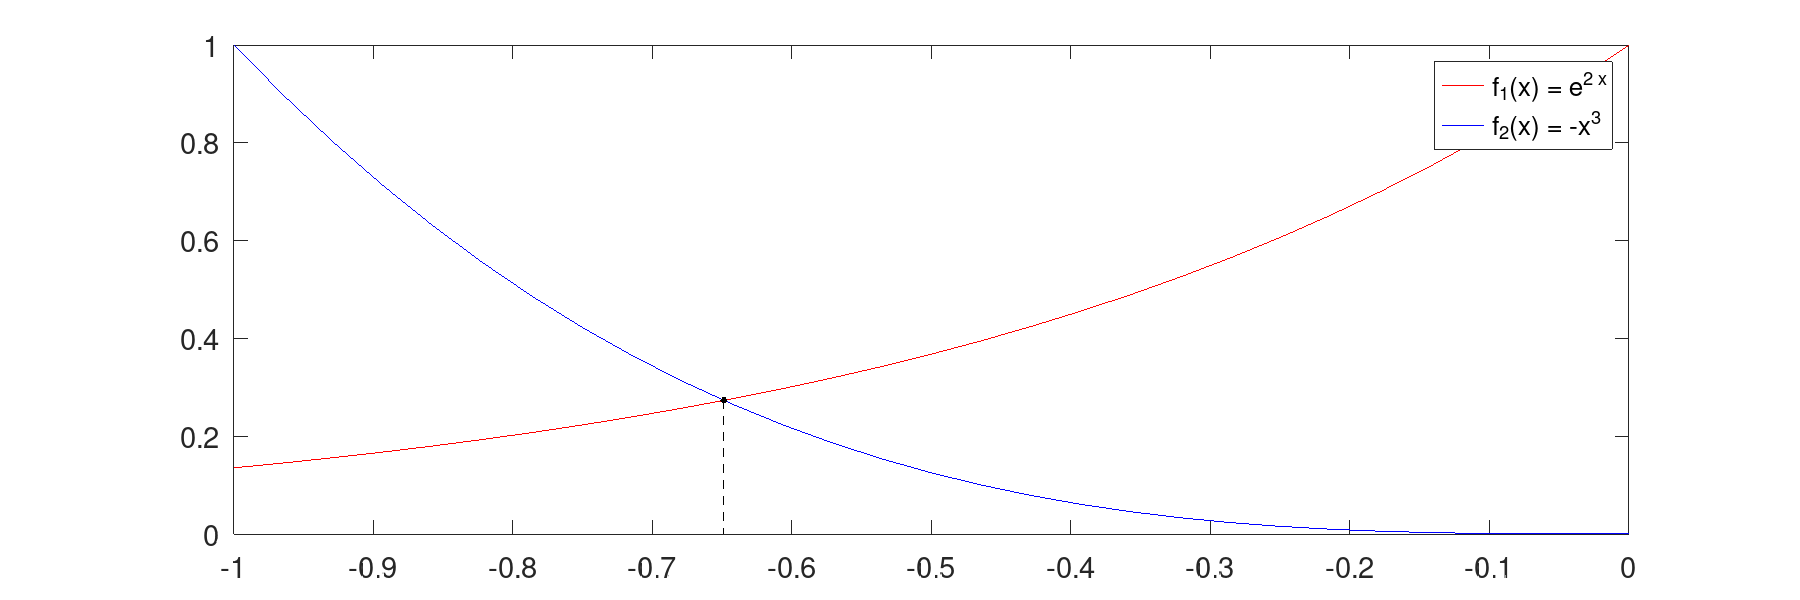
\includegraphics[width=\textwidth]{graphics/plot.png} 
  \caption{График функций \(f_1, f_2\) на промежутке \([-1, 0]\)}
\end{figure}

Проверим аналитически, что мы можем сузить рассматриваемую окрестность. По графику очевидно, что корень лежит рядом со значением \(-\frac{1}{2}\). Проверим саму эту точку:
\begin{align}\label{eq:right_border}
  f(-\frac{1}{2}) = e^{-1} - \frac{1}{8} > \frac{1}{3} - \frac{1}{8} > \frac{1}{8} - \frac{1}{8} = 0
\end{align}

За окрестность корня возьмем:
\begin{align}\label{eq:xi_nearby}
  U_\xi = \left[-1, -\frac{1}{2}\right]
\end{align}

В частности, выведем то, как ведет себя функция на границах и ровно в середине окрестности \eqref{eq:xi_nearby}. 
\begin{align} 
  \label{eq:dx_left_bound}
  f'(-1)  = \frac{2}{e^2} + 3 > \frac{2}{9} + 3 > 0 \\ 
  \label{eq:dx_middle_bound}
  f'\left(-\frac{1}{2}\right) = \frac{2}{e} + \frac{3}{4} > \frac{2}{3} + \frac{3}{4} > 0 \\ 
  \label{eq:dx_right_bound}
  f'\left(-\frac{3}{4}\right) = \frac{2}{\sqrt{e}^3} + \frac{9}{2} > \frac{2}{9} + \frac{9}{2} > 0 
\end{align}
Это было очевидно из сказанного \eqref{eq:df_geq}.

\subsubsection{Выпуклость}
Нам нужно еще убедиться в выпуклости функции в выбранной окрестности. Для того рассмотрим \(f''\):
\begin{align}
  f''(x) = 4e^{2x} + 6x
\end{align}

Эта функция есть сумма двух монотонно возрастающих функций, так что она сама по себе монотонно возрастает. Так что нам достаточно убедиться в одной границе и сравнить знаки.
Рассмотрим сразу середину заданного промежутка:
\begin{align}
  f''\left(-\frac{3}{4}\right) = 4 e^{-\frac{3}{2}} - \frac{9}{2} < 4 e^0 - \frac{9}{2} = 4 - \frac{9}{2} = -\frac{1}{2} < 0
\end{align}

Теперь, когда мы увидели значение \(f''\left(-\frac{3}{4}\right)\), а оно меньше нуля, мы можем с уверенностью сказать, что \(f''\) меньше нуля на всем начальном промежутке. Проверим остаток:
\begin{align}
  f''(-\frac{1}{2}) = 4 e^{-1} - 3 < 4 2^{-1} - 3 = 2 - 3 = -1 < 0 \label{eq:ddx_right}
\end{align}
Итак, \(f''\) меньше нуля и на остатке, да и вообще говоря на всем заданном промежутке \([-1, -\frac{1}{2}]\), что подтверждает выпуклость функции на этом участке и позволяет нам использовать метод Ньютона для поиска корня с уверенностью в его сходимости.

\subsubsection{Резюме}
Подытожим сказанное более строго. Мы отделили единственный корень нелинейного уравнения на \(\mathbb{R}\), задали для него окрестность в виде промежутка \([-1, -\frac{1}{2}]\). Для него было выявлено:
\begin{enumerate}
  \item На концах этого промежутка функция \(f\) принимает значения разного знака (\cref{eq:left_border,eq:right_border}). Она к тому же \(f \in C[-1, -\frac{1}{2}]\), так что есть корень \(\xi\), расположенный в этой окрестности;
  \begin{align*}
    f(-1) <  0 \\
    f\left(-\frac{1}{2}\right) > 0
  \end{align*}
  \item Оценки \cref{eq:dx_left_bound,eq:dx_middle_bound,eq:dx_right_bound} показывают, что функция монотонно возрастает --- это важно для итерационных методов нахождения корня;
\begin{align*} 
  f'(-1) > 0 \\ 
  f'\left(-\frac{1}{2}\right) > 0 \\ 
  f'\left(-\frac{3}{4}\right) > 0 
\end{align*}
  \item Оценки описанные в \cref{eq:ddx_right}:
    \begin{align*}
      f''(-\frac{1}{2}) < 0
    \end{align*} А также:
    \begin{align}
      f''(-1) = 4 e^{-2} - 6 < 4 e^0 - 6 = 4 - 6 = -2
    \end{align}
    и общие соображения насчет поведения функции \(f''\) показывают, что на заданном промежутке функция выпукла. Это понадобится для метода Ньютона.
\end{enumerate}

\begin{remark}[точность \(\varepsilon = 10^{-5}\)] {Вычисленные оценки}
  \begin{enumerate}
    \item Значения \cref{eq:left_border,eq:right_border}:
      \begin{align*}
        &f(-1) = e^{-2} - 1 \approx -\frac{552099556}{638512875} = -0.8646647195641905 \approx -0.86466 \\
        &f(-\frac{1}{2}) = e^{-1} - \frac{1}{8} \approx \frac{1399}{5760} = 0.2428819444444444 \approx 0.24288
      \end{align*}
    \item Значения \cref{eq:dx_left_bound,eq:dx_middle_bound,eq:dx_right_bound}:
      \begin{align*}
        &f'(-1) = 2 e^{-2} + 3 \approx \frac{2088365263}{638512875} = 3.2706705608716189 \approx 3.27067 \\
        &f'(-\frac{1}{2}) = 2 e^{-1} + \frac{3}{4} \approx \frac{33697}{22680} = 1.485758377425044 \approx 1.48575 \\
        &f'(-\frac{3}{4}) = 2 e^{-\frac{3}{4}} + \frac{27}{16} \approx \frac{1254202472387}{587789762560} = 2.133760320908914 \approx 2.13376
      \end{align*}
    \item Значение \cref{eq:ddx_right}:
      \begin{align*}
        f''(-\frac{1}{2}) = 4 e^{-1} - 3 \approx -\frac{35692090019}{23351328000} = -1.528482235314411 \approx -1.52848
      \end{align*}
  \end{enumerate}
\end{remark}

